\documentclass[tikz,border=2pt]{standalone}
\usepackage{amsmath}


\begin{document}

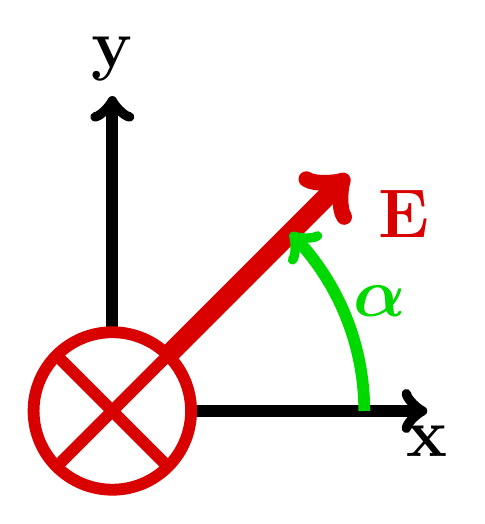
\begin{tikzpicture}

\draw[color=black,line width=1.5mm,->] (1.0,0.0) -- (4,0) 
node[anchor=north] {\Huge $\mathbf{x}$};
\draw[color=black,line width=1.5mm,->] (0.0,1.0) -- (0,4) 
node[anchor=south] {\Huge $\mathbf{y}$};
\draw[color=black!15!red,line width=2.5mm,->] (0.7,0.7) -- (3,3);
\draw[thick,color=black!15!red] (3.7,3.7);
\draw[color=black!15!red] (3.7,2.5) node[] {\Huge $\mathbf{E}$};
\draw[color=black!15!red,line width=1.5mm,-] 
(-0.7,-0.7) --(0.7,0.7);
\draw[color=black!15!red,line width=1.5mm,-] 
(0.7,-0.7) --(-0.7,0.7);
\draw[color=black!15!red,line width=1.5mm,->] (0,0) circle (1cm);
\draw [color=black!15!green,thick,domain=0:45,line width=1.5mm,->] 
plot ({3.2*cos(\x)}, {3.2*sin(\x)});
\draw[color=black!15!green] (3.4,1.4) node[] {\Huge $\boldsymbol{\alpha}$};

\end{tikzpicture}

\end{document}
